
\documentclass[template=tabling,81pt,headonall]{azmoon}
\usepackage{xepersian}
\usepackage{amsfonts}
\usepackage{graphicx}
\graphicspath{ {./images/} }
\settextfont{Yas}
\setdigitfont{A Iranian Sans}
\usepackage{fontawesome5}

\printanswers
    \teacher{محمد صالح علی اکبری}
    \teachertitle{دبیر}
    \city{گناباد}
    \schooltitle{متوسطه دوره دوم}
    \school{شاهد امام (ره)}
    \grade{دهم}
    \branch{۱۵۱}
    \topic{ریاضی}
    \examdate{۱۴۰۲/۱۰/۰۴}
    \answertime{80 دقیقه}
    \begin{document}
	\begin{questions}
		\nointerlineskip%
		\vskip-\baselineskip
		\question[0.5]{%
نقیض گزاره زیر را بنویسید.
    \begin{parts}[1]\part{عدد $\sqrt{2}$ گنگ است.}
\end{parts}

    }\question[1]{%
برای هر یک از گزاره‌های زیر مثال نقضی ارائه کنید.
    \begin{parts}[1]\part{تمام اعضای مجموعه $\{2k +1|k \in \mathbf{Z} \}$ زوج هستند.}
\part{عمود منصف‌های هر دو وتر از یک دایره فقط در مرکز دایره هم دیگر را قطع می‌کنند.}
\end{parts}

    }\question[1.5]{%
اثبات کنید $\sqrt{2}$ گنگ است. (راهنمایی از برهان خلف استفاده کنید.) \\}\question[2]{%
در شکل زیر اثبات کنید نسبت مساحت مثلث ACD به ABC برابر $\dfrac{3}{2}$. (خط d با پاره خط BC موازی است. $\dfrac{AD}{BC}=\dfrac{3}{2}$) \\ 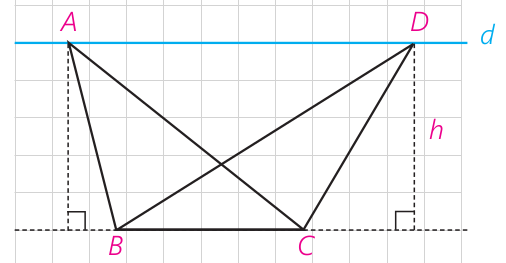
\includegraphics[scale = 0.31]{Screenshot from 2023-12-25 06-17-21}}\question[2]{%
صورت قضیه تالس را بنویسید و اثبات کنید. \\ \\ \\ \\}\question[2]{%
اگر خطی دو ضلع مثلثی را در دو نقطه قطع کند و با ضلع سوم آن موازی باشد، مثلثی پدید می‌آید که اندازه ضلع‌های آن با اندازه ضلع‌های ملث اصلی متناسب اندک مثلا در شکل زیر داریم:\\$\dfrac{AD}{AB}=\dfrac{AE}{AC}=\dfrac{DE}{BC}$\\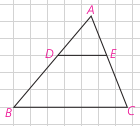
\includegraphics[scale = 1]{Screenshot from 2023-12-25 06-07-15} \\در شکل مقابل، $MNQB$ متوازی‌الضلاع است. اگر مساحت مثلث $PNM$، $60$ درصد مساحت مثلث $AMN$ باشد، نسبت $QC$ به $MN$ را محاسبه کنید. \\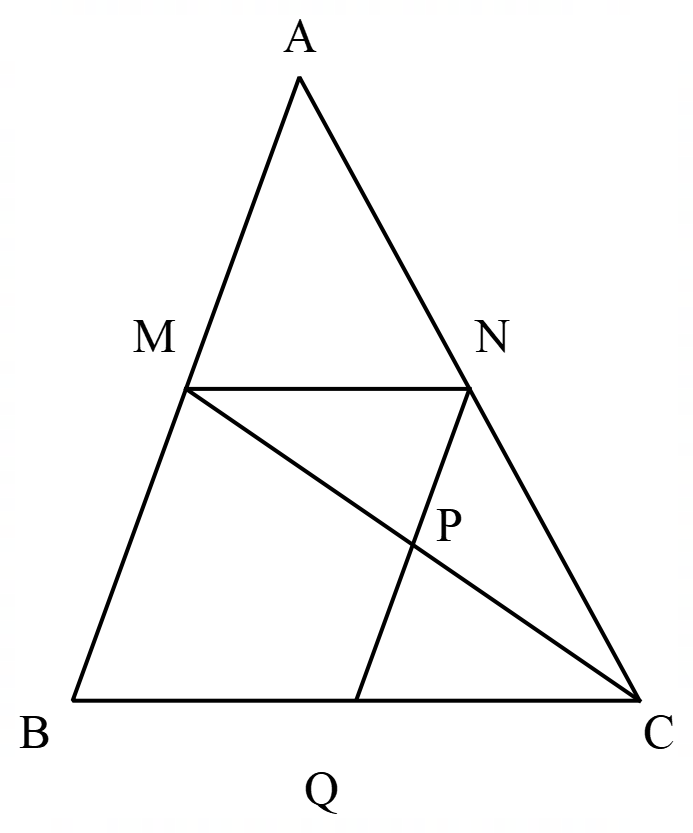
\includegraphics[scale = 0.8]{تالس خاص}}\end{questions}
    \end{document}
    